\documentclass[12pt, twoside, a4paper]{article}

\usepackage{booktabs}
\usepackage[sort&compress]{natbib}
\usepackage{pdfpages}

\linespread{1.5}

\begin{document}

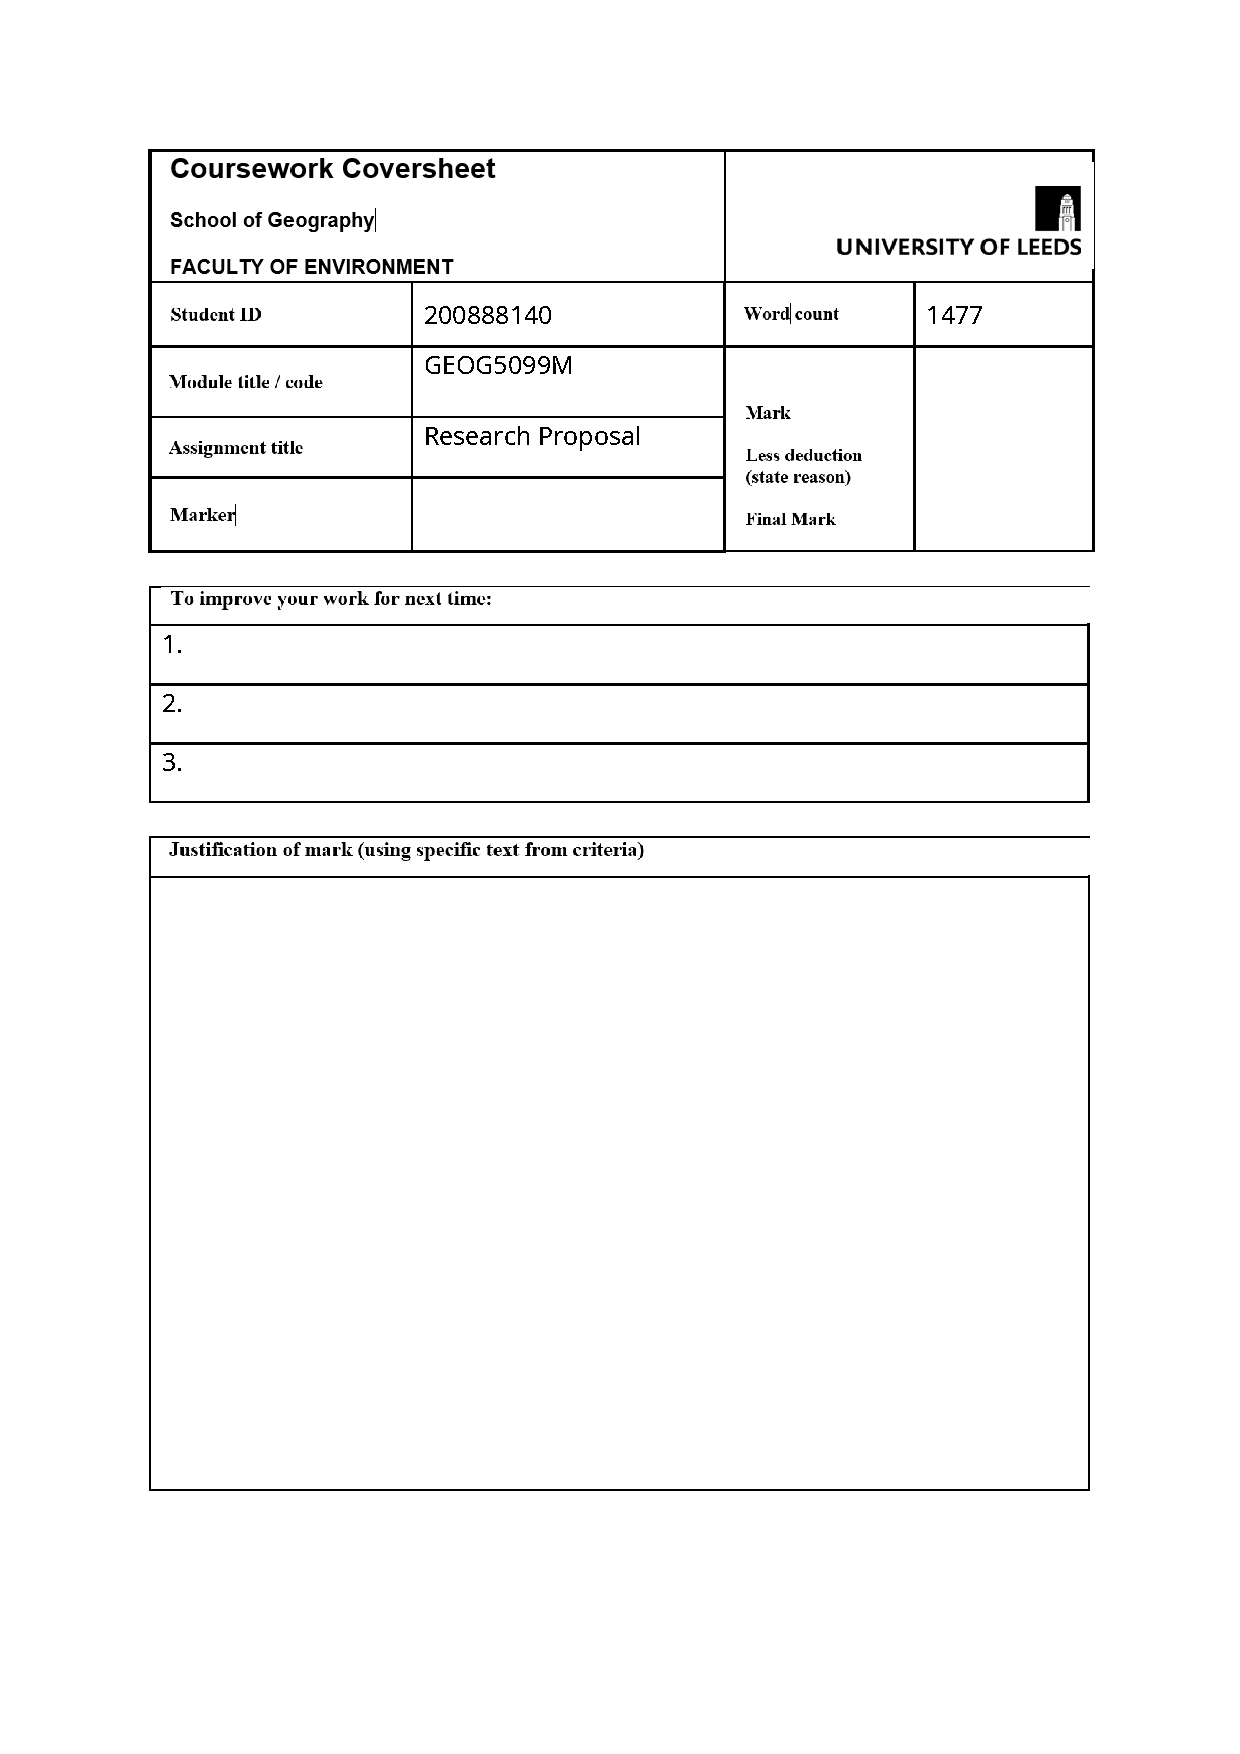
\includepdf[pages=-]{cover_sheet.pdf}

\title{Research Proposal}
\author{Keiran Suchak --- 200888140}
\maketitle

\section{Title of Research Topic}\label{sec:title}

Real-time Pedestrian Modelling: Implementing the Ensemble Kalman Filter for an
Agent-Based Model

\section{Research Questions and Statement}\label{sec:questions}

%The research questions and statement should drop out and emerge from the review of the literature and the description of the topic in section b. 
%Essentially this is an evaluation of how well the student has been able to distil the research into a set of solid research questions. 

The work undertaken in this dissertation seeks to address the following research
question: Can the Ensemble Kalman Filter method of data assimilation be used to
improve the accuracy with which an agent-based model simulates pedestrian
movement given observational data.
The Ensemble Kalman Filter is a method of combining two streams of
data; in our case, we aim to combine the states predicted by our pedestrian
model with synthetic data as a proof of concept.

In order to answer the above question, the following objectives are set out:
\begin{enumerate}
    \item Develop a general Ensemble Kalman Filter computational class.
    \item Apply the Ensemble Kalman Filter to our pedestrian model.
    \item Compare the accuracy with which the Ensemble Kalman Filter
        implementation of the model simulates the pedestrian movement against
        the base model without data assimilation.
\end{enumerate}

\section{Description of Research}\label{sec:research_descr}

%This section should describe the background to the research topic, provide a review of the relevant literature (methodological and or previous work in this domain) and should point towards research gaps that will be addressed by this thesis. 
%Essentially the student is being asked to demonstrate their understanding of the topic area, to show that they can summarise a body of research and to develop an implicit rationale for the need for their proposed research.

Knowledge of how people move around their environment can be made use of by both
academics and policy-makers in the contexts of urban planning, event management
and emergency response, particularly when considering urban environments.
Furthermore, such knowledge may be of use to those interested in the social issues of
mobility, inclusivity and accessibility of opportunities.

When considering such concepts, investigators often make use of modelling
techniques.
At their most fundamental, models represent our understanding of the system that
we are studying --- an understanding that may not be perfect
\citep{stanislaw1986tests}.
Whilst there exist modelling techniques for the simulation of how pedestrians
move around urban spaces, they exist largely in isolation of the real-world --- that is
to say that whilst the simulations aim to reflect the real-world, there is no
method by which we can incorporate up-to-date observations into these models to
stop their divergence from reality.

Simulating pedestrian behaviour is often undertaken at a micro-scale, with such
models typically aiming to model at the individual level or on a spatially
fine-grained grid \citep{burstedde2001simulation}.
One of the most prevalent simulation methods in this field is that of
Agent-Based Modelling.
Such methods consist of two key components: agents and environments.
In an Agent-Based Model, we prescribe sets of rules by which individuals
interact with each other and their local environment; as interactions take
place on the micro-scale, we typically observe the emergence of structure at the
macro-scale such as crowding \citep{batty2003discrete} or lane formation
\citep{liu2014agent}.
The evaluation of these rules is often not deterministic and instead introduces
some element of randomness; these stochastic elements aim to emulate the
variability of human behaviour.
The introduction of such randomness in conjunction with an imperfect
understanding of the phenomena at play, however, typically result in simulation
runs diverging from the real system.

In constructing their models, agent-based modellers undertake a development
process that involves model verification \citep{xiang2005verification},
validation \citep{crooks2008key} and calibration \citep{thiele2014facilitating}.
Beyond this, modellers also make efforts to ensure that the initial model
conditions are realistic by setting them based on historical data.

The practices of validation, calibration and setting initial model states based
on historical data are appropriate for offline evaluations such as testing
designs of new buildings or experimenting with different individual behaviours;
however, when aiming to simulate events in real-time, this simply delays the
inevitable divergence of the model from the real system.
Furthermore, model parameters may be transient and thus require updating as
time passes and the dynamics evolve.

Given the apparently inevitable divergence of stochastic simulations from the
real system that they aim to model, one may alternatively turn to big data.
Data is now being generated in higher volumes and at greater velocity than ever
before \citep{chen2014big}; however there also exist issues with observational
data from such systems.
Whilst models typically allow us to simulate a whole system, observations are
typically sparse in either time or space (or both); this is to say that
observations rarely provide complete coverage of events.
We therefore seek a solution whereby we can integrate up-to-date observations
into our models as the models continue to simulate the system.

One of the methods by which we can combine knowledge represented by our model
with observations as they become available is through data assimilation
techniques, which are most commonly used in the field of numerical weather
prediction \citep{kalnay2003atmospheric}.
Such techniques are typically made up of two steps:
\begin{enumerate}
    \item \textbf{Predict}: Run the model forward, estimating the state of the
        system, until new observations become available.
    \item \textbf{Update}: Upon receipt of new observations, combine the model's
        estimate of the system state with the new data.
\end{enumerate}
These steps are repeated iteratively in a cycle.
It is important to note that just as there is error associated with the model,
we also acknowledge that there is observational error associated with the data.
The aim of incorporating the observations into the model is to improve the model
accuracy with respect to the true system.

A large volume of work exists in which such techniques are applied to
meteorological systems where the models are based on differential equations.
Significantly less work exists in which data assimilation methods are applied to
agent-based models \citep{wang2017random} --- in particular pedestrian models
\citep{wang2013data, rai2013behavior, wang2015data, ward2016dynamic}.
Of the aforementioned studies, \citet{wang2013data}, \citet{rai2013behavior} and
\citet{wang2015data} focus on implementing a data assimilation scheme known as
the Particle Filter, whereas \citet{ward2016dynamic} focus on implementing
another scheme known as the Ensemble Kalman Filter to a very simple model;
indeed, the latter piece of work admits that the model used is ``relatively
simple in comparison with typical ABMs and is not programmed in an object
orientated framework''.
This dissertation therefore aims to expand on the pre-existing work by
implementing the Ensemble Kalman Filter in conjunction with an agent-based model
of pedestrians crossing a two-dimensional station from one side to the other.

\section{Description of Methodology and Data}\label{sec:method_descr}

%This section should describe the data and methods that will be used as part of this study. 
%The student should show their understanding of how the data analysis will allows the research aims / questions will be answered. 
%The data should exist, it should be available to the study within the proposed timeframe, indications of communications between data holders and students should be included, and a realistic appraisal of contingency data should be considered.

%\begin{itemize}
    %\item Data assimilation generally
    %\item Ensemble Kalman Filter
    %\item What data is used? Synthetic data from the model
    %\item What is the model?
%\end{itemize}

This dissertation focuses on the application of data assimilation schemes to
agent-based models, in particular considering the Ensemble Kalman Filter (EnKF),
which is a method derived from the Kalman Filter (KF).
The aim of the KF is to combine two streams of information based on their
uncertainties in order to produce an estimate for which the uncertainty is
minimised \citep{kalman1960new}.
In doing so, it sequentially evolves the state and the covariance matrix (which
characterises the state uncertainty).
It provides an optimal solution in scenarios that fulfil the following
conditions \citep{mandel2009brief}:
\begin{itemize}
    \item The model is linear,
    \item The uncertainties are normally distributed.
\end{itemize}

These criteria are not always fulfilled; indeed, when considering agent-based
models, we often find that the models are non-linear.
Furthermore, as models grow in dimension, so does the cost of evolving the
covariance matrix --- this quickly becomes intractable for larger models.

In order to address some of these issues, the Ensemble Kalman Filter was
developed \citep{evensen2003ensemble, evensen2009ensemble}.
Critically, this approach allows us to maintain a non-linear model
\citep{wikle2007bayesian}.
The EnKF acts as an approximation of the KF.
This approximation is achieved by using an ensemble of sample state vectors to
represent the state distribution.
As such, the model state is represented by a matrix, $\mathbf{X}$, as follows:
\begin{equation}
    \mathbf{X} = \left[ \mathbf{x}_1, \ldots, \mathbf{x}_N \right],
\end{equation}
where the state ensemble matrix, $\mathbf{X}$, consists of $N$ state vectors,
$\mathbf{x}_i$ ($\forall i \in (1, N)$.
Similarly, the observations are represented by a matrix, $\mathbf{D}$, as
follows:
\begin{equation}
    \mathbf{D} = \left[ \mathbf{d}_1, \ldots, \mathbf{d}_N \right],
\end{equation}
with each member of the data ensemble matrix, $\mathbf{D}$, being the sum of the
original observation, $\mathbf{d}$, and a random vector,
$\mathbf{\varepsilon}_i$:
\begin{equation}
    \mathbf{d}_i = \mathbf{d} + \mathbf{\varepsilon}_i.
\end{equation}
The random vector is drawn from an unbiased normal distribution:
\begin{equation}
    \mathbf{\varepsilon} \sim \mathcal{N} 
                              \left( 0, \mathbf{R} \right),
\end{equation}
where $\mathbf{R}$ is the data covariance matrix, representing the uncertainty
in the observations.

The state of the system, $\mathbf{X}$, is iteratively forecast by the model until
new observations are received; upon receipt of new data, the updated state
ensemble matrix, $\hat{\mathbf{X}}$, is given by:
\begin{equation}
    \hat{\mathbf{X}} = \mathbf{X} + \mathbf{K}
                       \left(
                       \mathbf{D} - \mathbf{H} \mathbf{X}
                       \right),
\end{equation}
where $\mathbf{K}$ is known as the Kalman gain matrix and $\mathbf{H}$ is known
as the observation matrix.
The observation matrix is responsible for converting the model state into
observation state space.
The Kalman gain matrix dictates the weighting applied to difference between the
observations and the model state in updating the state, and is given by:
\begin{equation}
    \mathbf{K} = \mathbf{Q} \mathbf{H}^T
                 {\left(
                    \mathbf{H} \mathbf{Q} \mathbf{H}^T + \mathbf{R}
                 \right)} ^ {-1},
\end{equation}
where $\mathbf{Q}$ is the covariance matrix representing the uncertainty in the
model state.
The Kalman gain matrix therefore weights the update based on the proportion of
the total uncertainty contributed by the model uncertainty.

This scheme will be applied to an agent-based model which simulates the motions
of pedestrians moving in two dimensions across a station from one side to the
other
\footnote{https://github.com/Urban-Analytics/dust/tree/master/Projects/StationSim-py}.
The data used for assimilation will be synthetic, and will be generated by the
same model.

\section{Timetable of Programme of Work}\label{sec:timetable}

%This should show a realistic plan of work for an August / September submission.

The work for this dissertation will be undertaken based on the following
deadlines:
\begin{itemize}
    \item \textbf{6th May 2019}: Write code for general Ensemble Kalman Filter.
    \item \textbf{15th May 2019}: Test Ensemble Kalman Filter on pedestrian model.
    \item \textbf{24th May 2019}: First draft of dissertation.
    \item \textbf{14th June 2019}: Complete dissertation.
\end{itemize}

\section{Risk Assessment}\label{sec:risk_ass}

The following factors are perceived to be risks to the success of the project:
\begin{itemize}
    \item Time constraints (low risk, high impact): Plan to submit dissertation well in
        advance, allowing plenty of time for any exceptional circumstances.
    \item Lack of available data (low risk, high impact): Using synthetic data
        from the pedestrian model, which are easily generated.
    \item Lack of computing resources (low risk, medium impact): Initial test
        indicate that code can be run on laptops; previous arrangements have
        been made for access to the SEE server which provides a significant
        boost in computational performance if required.
\end{itemize}

%This should be a general assessment of the possible risks, their likelihood, the strength of their impact and any possible mitigation strategies. 
%Obviously not every eventuality can be considered but general risks to the successful completion of the project should be identified and considered.

\bibliographystyle{agsm}
\bibliography{references}

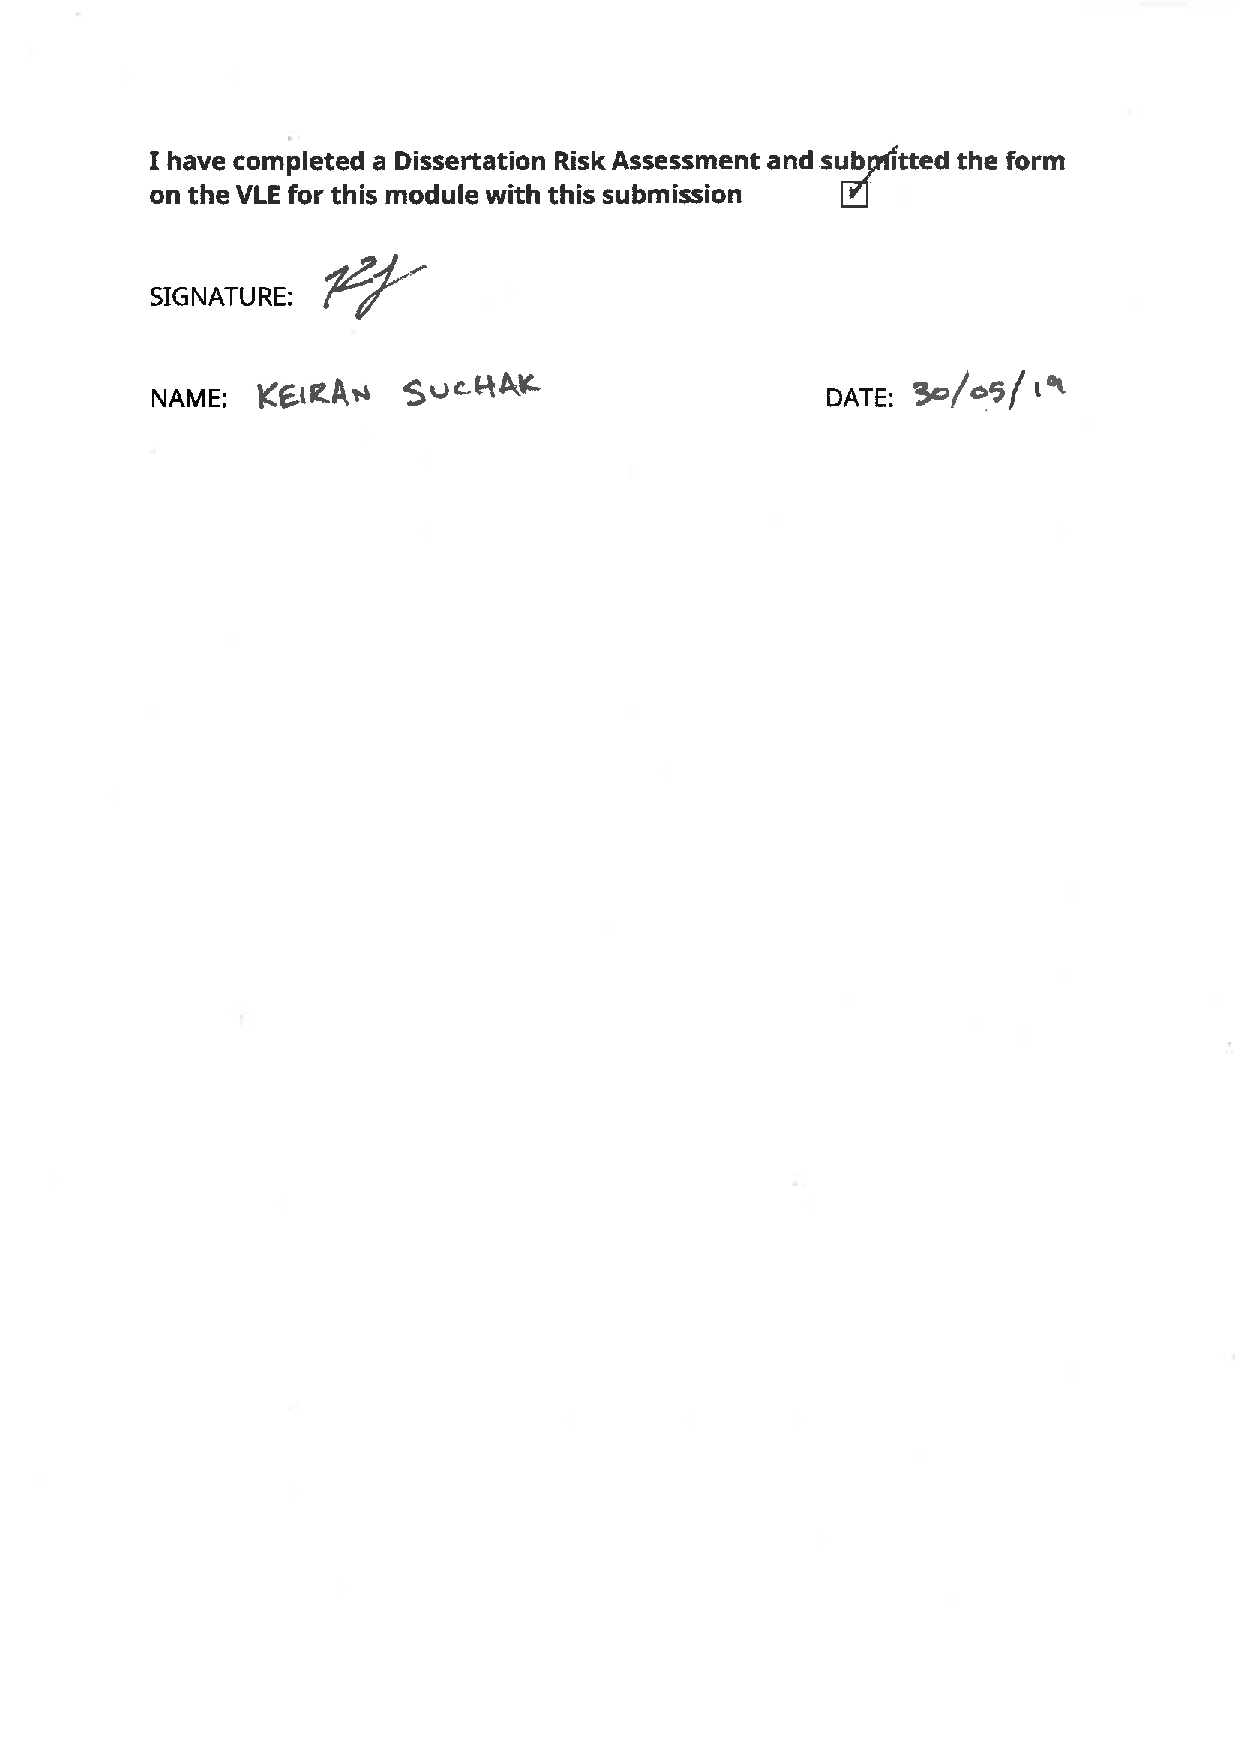
\includepdf[pages=-]{risk_declaration_filled.pdf}


\end{document}
